%% abtex2-modelo-artigo.tex, v-1.9.7 laurocesar
%% Copyright 2012-2018 by abnTeX2 group at http://www.abntex.net.br/ 
%%
%% This work may be distributed and/or modified under the
%% conditions of the LaTeX Project Public License, either version 1.3
%% of this license or (at your option) any later version.
%% The latest version of this license is in
%%   http://www.latex-project.org/lppl.txt
%% and version 1.3 or later is part of all distributions of LaTeX
%% version 2005/12/01 or later.
%%
%% This work has the LPPL maintenance status `maintained'.
%% 
%% The Current Maintainer of this work is the abnTeX2 team, led
%% by Lauro César Araujo. Further information are available on 
%% http://www.abntex.net.br/
%%
%% This work consists of the files abntex2-modelo-artigo.tex and
%% abntex2-modelo-references.bib
%%

% ------------------------------------------------------------------------
% ------------------------------------------------------------------------
% abnTeX2: Modelo de Artigo Acadêmico em conformidade com
% ABNT NBR 6022:2018: Informação e documentação - Artigo em publicação 
% periódica científica - Apresentação
% ------------------------------------------------------------------------
% ------------------------------------------------------------------------

\documentclass[
% -- opções da classe memoir --
article,			% indica que é um artigo acadêmico
11pt,				% tamanho da fonte
oneside,			% para impressão apenas no recto. Oposto a twoside
a4paper,			% tamanho do papel. 
% -- opções da classe abntex2 --
%chapter=TITLE,		% títulos de capítulos convertidos em letras maiúsculas
%section=TITLE,		% títulos de seções convertidos em letras maiúsculas
%subsection=TITLE,	% títulos de subseções convertidos em letras maiúsculas
%subsubsection=TITLE % títulos de subsubseções convertidos em letras maiúsculas
% -- opções do pacote babel --
english,			% idioma adicional para hifenização
brazil,				% o último idioma é o principal do documento
sumario=tradicional,
]{abntex2}


% ---
% PACOTES
% ---

% ---
% Pacotes fundamentais 
% ---
\usepackage{lmodern}			% Usa a fonte Latin Modern
\usepackage[T1]{fontenc}		% Selecao de codigos de fonte.
\usepackage[utf8]{inputenc}		% Codificacao do documento (conversão automática dos acentos)
\usepackage{indentfirst}		% Indenta o primeiro parágrafo de cada seção.
\usepackage{nomencl} 			% Lista de simbolos
\usepackage{color}				% Controle das cores
\usepackage{graphicx}			% Inclusão de gráficos
\usepackage{microtype} 			% para melhorias de justificação
% ---

% ---
% Pacotes adicionais, usados apenas no âmbito do Modelo Canônico do abnteX2
% ---
\usepackage{lipsum}				% para geração de dummy text
% ---

% ---
% Pacotes de citações
% ---
\usepackage[brazilian,hyperpageref]{backref}	 % Paginas com as citações na bibl
\usepackage[alf]{abntex2cite}	% Citações padrão ABNT
% ---

% ---
% Configurações do pacote backref
% Usado sem a opção hyperpageref de backref
\renewcommand{\backrefpagesname}{Citado na(s) página(s):~}
% Texto padrão antes do número das páginas
\renewcommand{\backref}{}
% Define os textos da citação
\renewcommand*{\backrefalt}[4]{
	\ifcase #1 %
	Nenhuma citação no texto.%
	\or
	Citado na página #2.%
	\else
	Citado #1 vezes nas páginas #2.%
	\fi}%
% ---

% --- Informações de dados para CAPA e FOLHA DE ROSTO ---
\titulo{ Comparação de indutores para modelos de predição de classifição de imagens }
\tituloestrangeiro{}

\autor{
	Lucas Mrowskovsy Paim\thanks{Programa de Pós Graduação em Inteligência Aritificial, Curitiba - PR, 80215-901; Especializando em Inteligência Artificial Aplicada na PUCPR; Tecnólogo em Sistemas para Internet pela Universidade Positivo; E-mail: lucasmpaim1@gmail.com} }
\local{Brasil}
\data{2019}
% ---

% ---
% Configurações de aparência do PDF final

% alterando o aspecto da cor azul
\definecolor{blue}{RGB}{41,5,195}

% informações do PDF
\makeatletter
\hypersetup{
	%pagebackref=true,
	pdftitle={\@title}, 
	pdfauthor={\@author},
	pdfsubject={Modelo de artigo científico com abnTeX2},
	pdfcreator={LaTeX with abnTeX2},
	pdfkeywords={abnt}{latex}{abntex}{abntex2}{atigo científico}, 
	colorlinks=true,       		% false: boxed links; true: colored links
	linkcolor=blue,          	% color of internal links
	citecolor=blue,        		% color of links to bibliography
	filecolor=magenta,      		% color of file links
	urlcolor=blue,
	bookmarksdepth=4
}
\makeatother
% --- 

% ---
% compila o indice
% ---
\makeindex
% ---

% ---
% Altera as margens padrões
% ---
\setlrmarginsandblock{3cm}{3cm}{*}
\setulmarginsandblock{3cm}{3cm}{*}
\checkandfixthelayout
% ---

% --- 
% Espaçamentos entre linhas e parágrafos 
% --- 

% O tamanho do parágrafo é dado por:
\setlength{\parindent}{1.3cm}

% Controle do espaçamento entre um parágrafo e outro:
\setlength{\parskip}{0.2cm}  % tente também \onelineskip

% Espaçamento simples
\SingleSpacing


% ----
% Início do documento
% ----
\begin{document}
	
	% Seleciona o idioma do documento (conforme pacotes do )
	%\selectlanguage{english}
	\selectlanguage{brazil}
	
	% Retira espaço extra obsoleto entre as frases.
	\frenchspacing 
	
	% ----------------------------------------------------------
	% ELEMENTOS PRÉ-TEXTUAIS
	% ----------------------------------------------------------
	
	%---
	%
	% Se desejar escrever o artigo em duas colunas, descomente a linha abaixo
	% e a linha com o texto ``FIM DE ARTIGO EM DUAS COLUNAS''.
	% \twocolumn[    		% INICIO DE ARTIGO EM DUAS COLUNAS
	%
	%---
	
	% página de titulo principal (obrigatório)
	\maketitle
	
	
	% titulo em outro idioma (opcional)
	
	
	
	% resumo em português
	\begin{resumoumacoluna}
		Este trabalho tem por objetivo comparar os indutores apresentados durante a disciplina de Machine Learning do programa de especialização em Inteligência Artificial Aplicada da Pontifícia Universidade Católica do Paraná, para predição de classificação de imagens, utilizando principalmente a bilioteca scikit-learn e a linguagem Python, assim como a demonstração de técnicas de combinação de indicadores e seleção dinâmica.

		Tem por objetivo também a comparação dos resultados utilizando técnicas de extração de características manuais, handcrafted, e CNN deep-learning.

		Para a extração de características de imagens foram utilizados as bibliotecas: opencv-python, skimage e keras

		//Falta a conclusão
		
		\vspace{\onelineskip}
		
		\noindent
		\textbf{Palavras-chave}: Naive Bayes. Árvores de decisão. Redes Neurais. k-Vizinhos Mais Próximos. Máquina de Vetores de Suporte.
	\end{resumoumacoluna}
	
	
	% resumo em inglês
	\renewcommand{\resumoname}{Abstract}
	\begin{resumoumacoluna}
		\begin{otherlanguage*}{english}
			This paper aims to compare the inductors presented during the Machine Learning discipline of the Pontifical Catholic University of Paraná specialization program in Applied Artificial Intelligence, to predict image classification using mainly the scikit-learn library and the Python language as well as the demonstration of techniques of combination of indicators and dynamic inductor selection.
			
			It also aims to compare the results using handcrafted and CNN deep-learning feature extraction techniques.
			
			For the extraction of image characteristics we used the libraries: opencv-python, skimage and keras.
			\vspace{\onelineskip}
			
			\noindent
			\textbf{Keywords}: Naive Bayes. Decision Tree. Neural Network. k-Nearest Neighbors. Support Vector Machine.
		\end{otherlanguage*}  
	\end{resumoumacoluna}
	
	% ]  				% FIM DE ARTIGO EM DUAS COLUNAS
	% ---
	
	
	%\begin{center}\smaller
	%	\textbf{Data de submissão e aprovação}: elemento obrigatório. Indicar dia, mês e ano
		
	%	\textbf{Identificação e disponibilidade}: elemento opcional. Pode ser indicado 
	%	o endereço eletrônico, DOI, suportes e outras informações relativas ao acesso.
	%\end{center}
	
	% ----------------------------------------------------------
	% ELEMENTOS TEXTUAIS
	% ----------------------------------------------------------
	\textual
	
	% ----------------------------------------------------------
	% Introdução
	% ----------------------------------------------------------
	\section{Introdução}
	
	A utilização de classificadores de imagens é utilizada nas mais diversas áreas do conhecimento,  que vão desde o auxílio de diagnóstico de câncer de pele  \citeonline{svm-cancer}, sistemas de segmentação e classificação de imagens via satélite \citeonline{seg-imagens-satelite}, OCR's (Optical Character Recognition) para reconhecimento de textos e dígitos \citeonline{ocr-digitos} etc.
	
	Os mesmos indutores também podem ser utilizados para outras finalidades que não sejam classificação de imagem, como: detecção de emoções em processamento de textos \citeonline{emocoes-em-texto}, regressão linear etc.
	
	Segundo \citeonline{benIA}, fornecer a capacidade de visão a sistemas computacionais, assim como a robôs, agentes é algo, sem dúvida, extremamente desejável.
	
	As técnicas de extração de caracterísicas de imagens handcrafted que foram utilizadas são: 
	
	\begin{itemize}
		\item LBP: Local Binnary Pattern: Segundo, \citeonline{lbp-opencv}, esta é uma técnica de extração de texturas de uma imagem, em que cada pixel é comparado com seus vizinhos a partir de uma máscara e com isso é gerado uma sequência binária que toma o lugar daquele pixel. 
		\item HOG: Histogram of Oriented Gradients: Segundo \citeonline{hog-opencv} é uma técnica de extrai a distribuição (Historgramas) de direções de gradientes.
		\item Histograma de Cores RGB.
	\end{itemize}
	
	
	% Visto o exposto o estudo desse trabalho se torna importante para ...., Podendo ser aplicado em diversas áreas, tendo por objetivo ...
	
	Visto o exposto o estudo desse trabalho se torna importante para a área de classifição de imagens, Podendo ser aplicado em diversas áreas, tendo por objetivo criar modelos de predição para classifição de imagens comparando vários indutores e os combinando para gerar maiores assertividades.
	
	
	\section{Método}
	
	
	A base utilizada para este trabalho, conta com apenas mil imagens, separadas em dez classes com cem imagens cada, sendo assim, é uma base completamente balanceada.
	
	Todos os indutores, foram treinados utilizando a mesma base de imagens, em um primeiro momento ela é separada em 70\%  em treinamento e 30\% em testes, técnica esta chamada de holdout (percentage-split), após esta separação ainda foi separado mais 30\% da base de treinamento e criada uma base de validação, para evitar assim o chamado overfitting, que segundo \citeonline{overfitting}, é um dos maiores problemas da aprendizagem de máquina, isto indica que o indutor está perdendo sua capacidade de generalização, isto é, segundo \citeonline{isIA} a capacidade do indutor responder adequadamente a dados que não fazem parte do conjunto de treinamento.
	
	Para a comparação dos indutores será avaliado, com base em holdout e também em validação cruzada que segundo, \citeonline{basic-concepts}, consiste em dividir a base de dados em N grupos, em que um desses grupos é selecionado para teste e isto é repetido N vezes, garantindo assim que todas as instâncias serão utilizadas como teste ao menos uma vez.
	
	Devido ao não suporte dos métodos de overfitting para alguns indicadores, este trabalho utiliza, quando disponível, o método:
	
	\begin{verbatim}
	.partial_fit(X, y, [classes])
	\end{verbatim}
	
	Este método segundo \citeonline{incremental-learning}, é ideal para treinamento incremental, sendo assim, é possível extender a lógica do early stopping para alguns indicadores que não suportam tal método nativamente, como o Naive Bayes.
	
	Como o método incremental, tende a adicionar ruído na base de dados, foi utilizado o método de IIR (Infinite Impulse Response), que segundo \citeonline{iir-concepts} é um filtro recursivo em que a saída do filtro é calculada usando as entradas atuais e anteriores e as saídas anteriores, fazendo assim com que o ruído seja minimizado, este filtro foi aplicado no tratamento de erro tanto da base de validação quanto da base de teste.
	
	Sua fórmula consiste em:
	
	\begin{equation}
	y_t = \sum_{i=0}^M b_jx_(t-i) - \sum_{j=1}^{L} \alpha_j y_(t-j)
	\end{equation}
	
	O resultado da aplicação desta técnica pode ser consultada na  \autoref{fig_smooth_example}, onde é possível observar que o gráfico foi suavizado, de forma que, quando ambas as bases forem confrontadas será possível detectar mais fácilmente onde está ocorrendo o overfitting.
	
	Sendo assim podemos definir a taxa de aprendizado como sendo:
	
	\begin{equation}
	r = {y_{t-1}} - {y_{t}}
	\end{equation}
	
	Onde \({y_{t-1}} \) se refere ao erro na base de validação na iteração anterior e \({y_t}\) se refere a iteração atual de treinamento, desta forma quando obtemos um valor para \(r < {10^{-3}}\) que é a taxa mínima de aprendizagem e isso ocorre por \(N\) vezes seguidas, significa que não há um ganho no treinamento e este pode ser interrompido.
 	
	\subsection{Naive Bayes}
	
	Segundo, \citeonline{naive-bayes-britto}, o teorema de Bayes consiste em uma abordagem probabilística para aprendizagem, calculando assim a probabilidade de uma característica \(X\) de um vetor de prever determinada classe.
	
	A técnica de Naive Bayes, assume que todas as caractéristicas no vetor são independentes, por isso, é chamado de Naive (do inglês Ingênuo), pois determinadas caracterísicas podem estar relacionadas entre si, o que faz com que essa técnica tenha um resultado inferior a ténica de Redes Bayesianas que consideram que os atributos podem ou não ser relacionados, isto é, a característica \(X\) pode ou não estar diretamente relacionada a característica \(Y\).
	
	\subsubsection{Resultados do Treinamento}
	
	A matriz de confusão para o esta técnica usando houldout e a base de características usando deeplearning pode ser consultada em \autoref{confusion-matrix-naive-holdout-deep}, assim como sua taxa de aprendizagem \autoref{error-naive-bayes-holdout}
	
	\begin{verbatim}
		Acurácia Naive Bayes Validação : 0.8928571428571429
		Acurácia Naive Bayes Teste     : 0.9266666666666666
	\end{verbatim}
	
	Para o método usando as características extraídas de forma hand crafting, a curva de erro na aprendizagem pode ser consultado na \autoref{error-naive-bayes-hand-craft-holdout}, assim como sua matriz de confução na \autoref{confusion-matrix-naive-holdout-hand-craft}.
	
	\begin{verbatim}
		Acurácia Naive Bayes Validação : 0.7785714285714286
		Acurácia Naive Bayes Teste     : 0.8533333333333334
	\end{verbatim}
	
	\subsection{Árvores de decisão}
	
	A técnica da árvore de decisão utiliza a teoria do ganho de informação (entropia) , para decidir seus novos vértices até que consiga realizar a classificação das instâncias.
	
	A entropia pode ser definida pela fórmula:
	
	\begin{equation}
	S = -p_+ log_2 p_+-p_-log_2p_-
	\end{equation}
	
	Onde \(p_+\) é a proporção de elementos positivos em \(S\) e \(p_-\) a de elementos negativos.
	
	 As árvores geradas para a este trabalho podem ser consultadas em: \autoref{decision-tree-holdout-deep}, \autoref{decision-tree-holdout-hand-craft}
	
	\subsubsection{Resultados do Treinamento}
	DEEP
	\begin{verbatim}
		Acurácia Decision Tree Teste     : 0.8466666666666667
	\end{verbatim}
	
	HAND-CRAFT
	\begin{verbatim}
	Acurácia Decision Tree Teste     : 0.67
	\end{verbatim}
	
	\subsection{Redes Neurais}
	
	\subsubsection{Resultados do Treinamento}
	DEEP
	\begin{verbatim}
	Acurácia Neural Network - adam Validação : 0.9357142857142857
	Acurácia Neural Network - adam Teste     : 0.92
	\end{verbatim}
	
	HAND-CRAFT
	\begin{verbatim}
	Acurácia Neural Network - adam Validação: 0.10714285714285714
	Acurácia Neural Network - adam Teste : 0.1
	\end{verbatim}
	
	\subsection{KNN}
	
	A técnica de k-nearest neighbors, k-vizinhos mais próximos, consiste em agrupar intâncias similares, e quando novas intâncias são inseridas para a classificação, elas são classificados pelos \(k\)-vizinhos mais próximos.
	
	Uma grande desvantagem desta abordagem que dispensa treinamento é que ela é mais lenta, uma vez que realiza todos os cálculos necessários a cada nova classificação
	
	\subsubsection{Resultados}
	
	DEEP	
	\begin{verbatim}
	Acurácia KNN Teste : 0.96
	\end{verbatim}
	
	HAND-CRAFT
	\begin{verbatim}
	Acurácia KNN Teste : 0.39666666666666667
	\end{verbatim}
	
	
	\subsection{SVM}
	A técnica de SVM consiste em "encontrar" novas dimensões para classificar os atríbutos
	\subsubsection{Resultado do Treinamento}
		
	DEEP	
	\begin{verbatim}
	Acurácia SVM Teste : 0.9833333333333333
	\end{verbatim}
	
	HAND-CRAFT
	\begin{verbatim}
	Acurácia SVM Teste : 0.7533333333333333
	\end{verbatim}
	
	% ---
	% Finaliza a parte no bookmark do PDF, para que se inicie o bookmark na raiz
	% ---
	\bookmarksetup{startatroot}% 
	% ---
	
	% ---
	% Conclusão
	% ---
	\section{Considerações finais}
	
	\lipsum[1]
	
	\begin{citacao}
		\lipsum[2]
	\end{citacao}
	
	\lipsum[3]
	
	% ----------------------------------------------------------
	% ELEMENTOS PÓS-TEXTUAIS
	% ----------------------------------------------------------
	\postextual
	
	% ----------------------------------------------------------
	% Referências bibliográficas
	% ----------------------------------------------------------
	\bibliography{references}
	
	% ----------------------------------------------------------
	% Glossário
	% ----------------------------------------------------------
	%
	% Há diversas soluções prontas para glossário em LaTeX. 
	% Consulte o manual do abnTeX2 para obter sugestões.
	%
	%\glossary
	
	% ----------------------------------------------------------
	% Apêndices
	% ----------------------------------------------------------
	
	% ---
	% Inicia os apêndices
	% ---
	\begin{apendicesenv}
		
		% ----------------------------------------------------------
		\chapter{Nullam elementum urna vel imperdiet sodales elit ipsum pharetra ligula
			ac pretium ante justo
		 a nulla curabitur tristique arcu eu metus}
		% ----------------------------------------------------------
		\lipsum[55-56]
		
	\end{apendicesenv}
	% ---
	
	% ----------------------------------------------------------
	% Anexos
	% ----------------------------------------------------------
	\cftinserthook{toc}{AAA}
	% ---
	% Inicia os anexos
	% ---
	%\anexos
	\begin{anexosenv}
		
		\begin{figure}[htb]
			\caption{\label{fig_smooth_example} Comparação do Erro com e sem IIR, usando Holdout}
			\begin{center}
				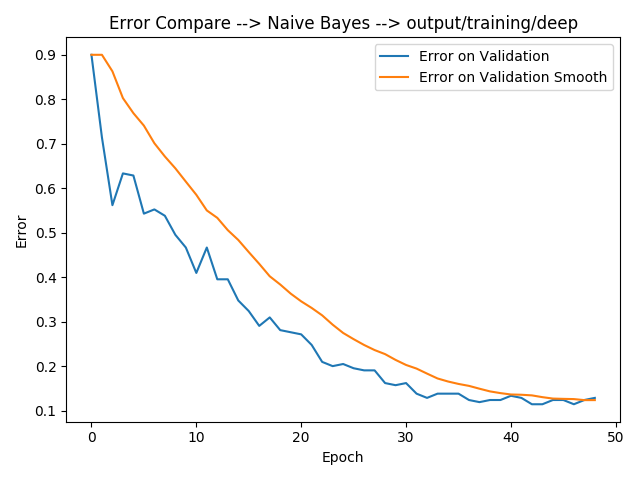
\includegraphics[scale=0.5]{smooth_compare.png}
			\end{center}
			\legend{Fonte: O Autor}
		\end{figure}
		
		\begin{figure}[htb]
			\caption{\label{error-naive-bayes-holdout}Gráfico de Margem de erro usando Holdout}
			\begin{center}
				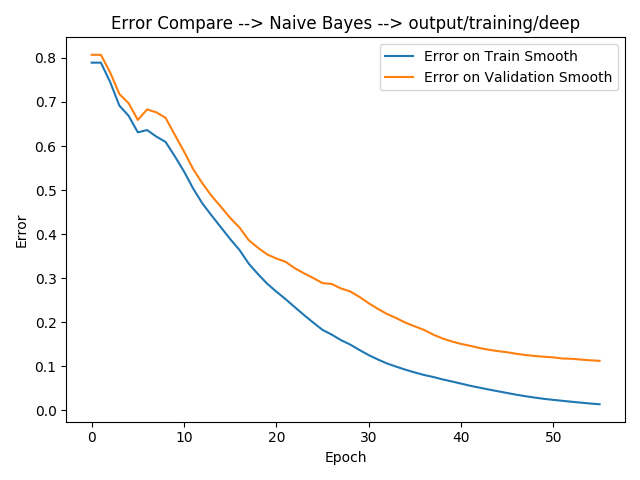
\includegraphics[scale=0.5]{error-naive-bayes-holdout.png}
			\end{center}
			\legend{Fonte: O Autor}
		\end{figure}

	
		\begin{figure}[htb]
			\caption{\label{confusion-matrix-naive-holdout-deep}Matrix de confusão Naive Bayes, usando Holdout}
			\begin{center}
				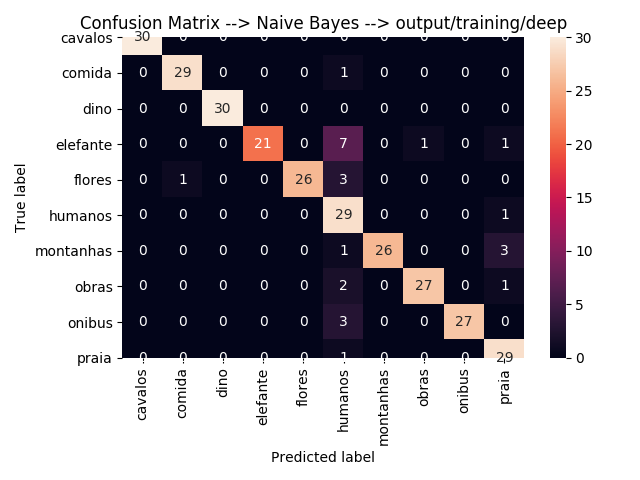
\includegraphics[scale=0.5]{confusion-matrix-naive-holdout-deep.png}
			\end{center}
			\legend{Fonte: O Autor}
		\end{figure}
	
		\begin{figure}[htb]
			\caption{\label{error-naive-bayes-hand-craft-holdout}Gráfico de treinamento Naive Bayes, usando Holdout}
			\begin{center}
				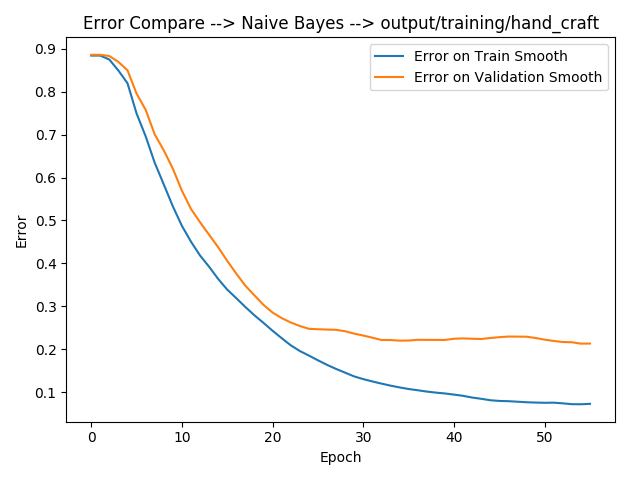
\includegraphics[scale=0.5]{error-naive-bayes-hand-craft-holdout.png}
			\end{center}
			\legend{Fonte: O Autor}
		\end{figure}
	
		\begin{figure}[htb]
			\caption{\label{confusion-matrix-naive-holdout-hand-craft}Matrix de confusão Naive Bayes, usando Holdout}
			\begin{center}
				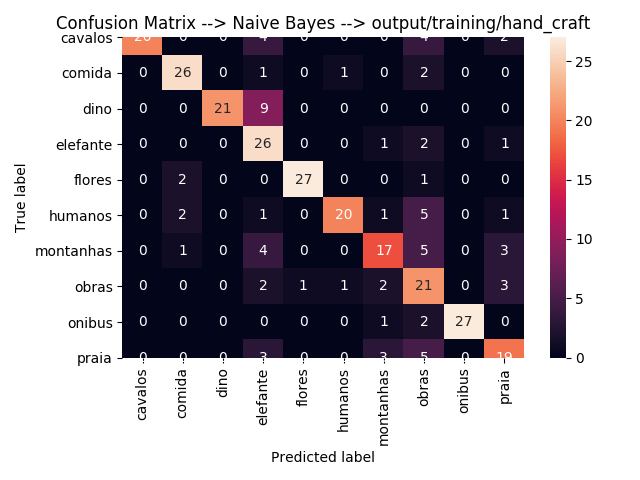
\includegraphics[scale=0.5]{confusion-matrix-naive-holdout-hand-craft.png}
			\end{center}
			\legend{Fonte: O Autor}
		\end{figure}
	
		\begin{figure}[htb]
			\caption{\label{decision-tree-holdout-deep}Decision Tree, usando Holdout e Deep Learning}
			\begin{center}
				
\includegraphics[scale=0.06]{Decision_Tree_Deep.pdf}
			\end{center}
			\legend{Fonte: O Autor}
		\end{figure}
	
	
	\begin{figure}[htb]
		\caption{\label{confusion-matrix-decision-tree-holdout-deep}Matrix de confusão Decision Tree, usando Holdout e Deep Learning}
		\begin{center}
			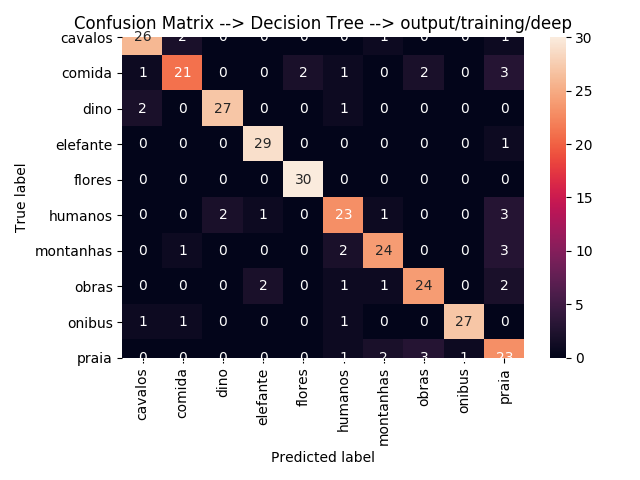
\includegraphics[scale=0.5]{confusion-matrix-decision-tree-deep.png}
		\end{center}
		\legend{Fonte: O Autor}
	\end{figure}
	
	\begin{figure}[htb]
		\caption{\label{decision-tree-holdout-hand-craft}Árvore de Desição, usando Holdout e Hand Craft}
		\begin{center}
			\includegraphics[scale=0.06]{Decision_Tree_Hand_Craft.pdf}
		\end{center}
		\legend{Fonte: O Autor}
	\end{figure}
	
	\begin{figure}[htb]
		\caption{\label{confusion-matrix-decision-tree-holdout-hand-craft}Matrix de confusão Decision Tree, usando Holdout e Hand Craft}
		\begin{center}
			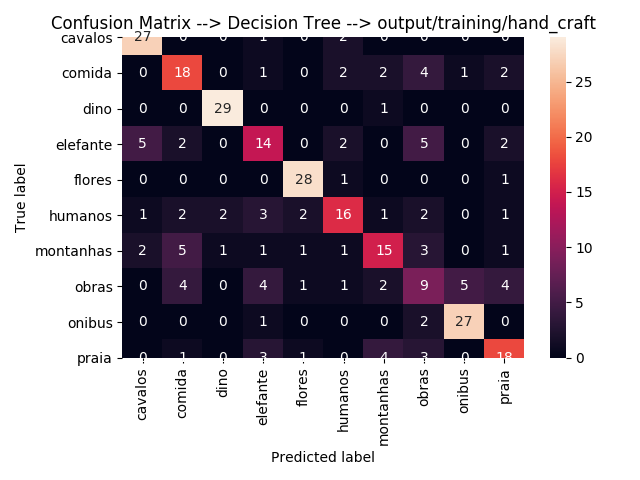
\includegraphics[scale=0.5]{confusion-matrix-decision-tree-holdout-hand-craft.png}
		\end{center}
		\legend{Fonte: O Autor}
	\end{figure}

	\begin{figure}[htb]
		\caption{\label{tsne-deep-data}TSNE Base Deep Learning}
		\begin{center}
			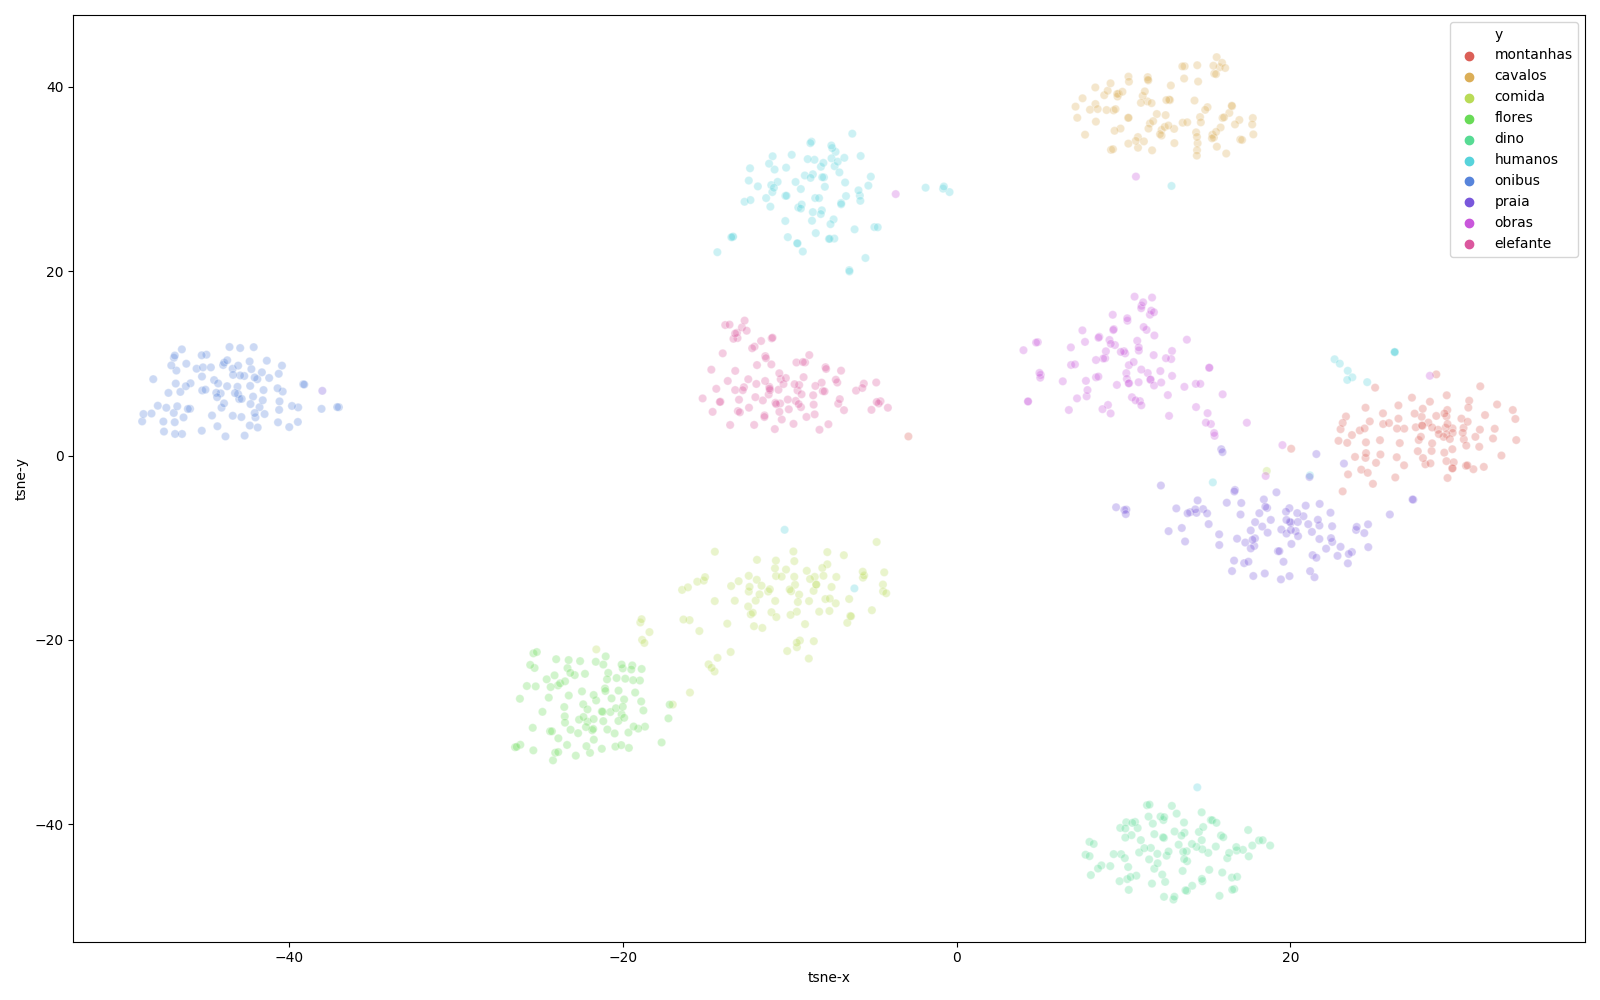
\includegraphics[scale=0.3]{tsne-graph-deep.png}
		\end{center}
		\legend{Fonte: O Autor}
	\end{figure}

	\begin{figure}[htb]
		\caption{\label{tsne-deep-data}TSNE Base Hand Crafting}
		\begin{center}
			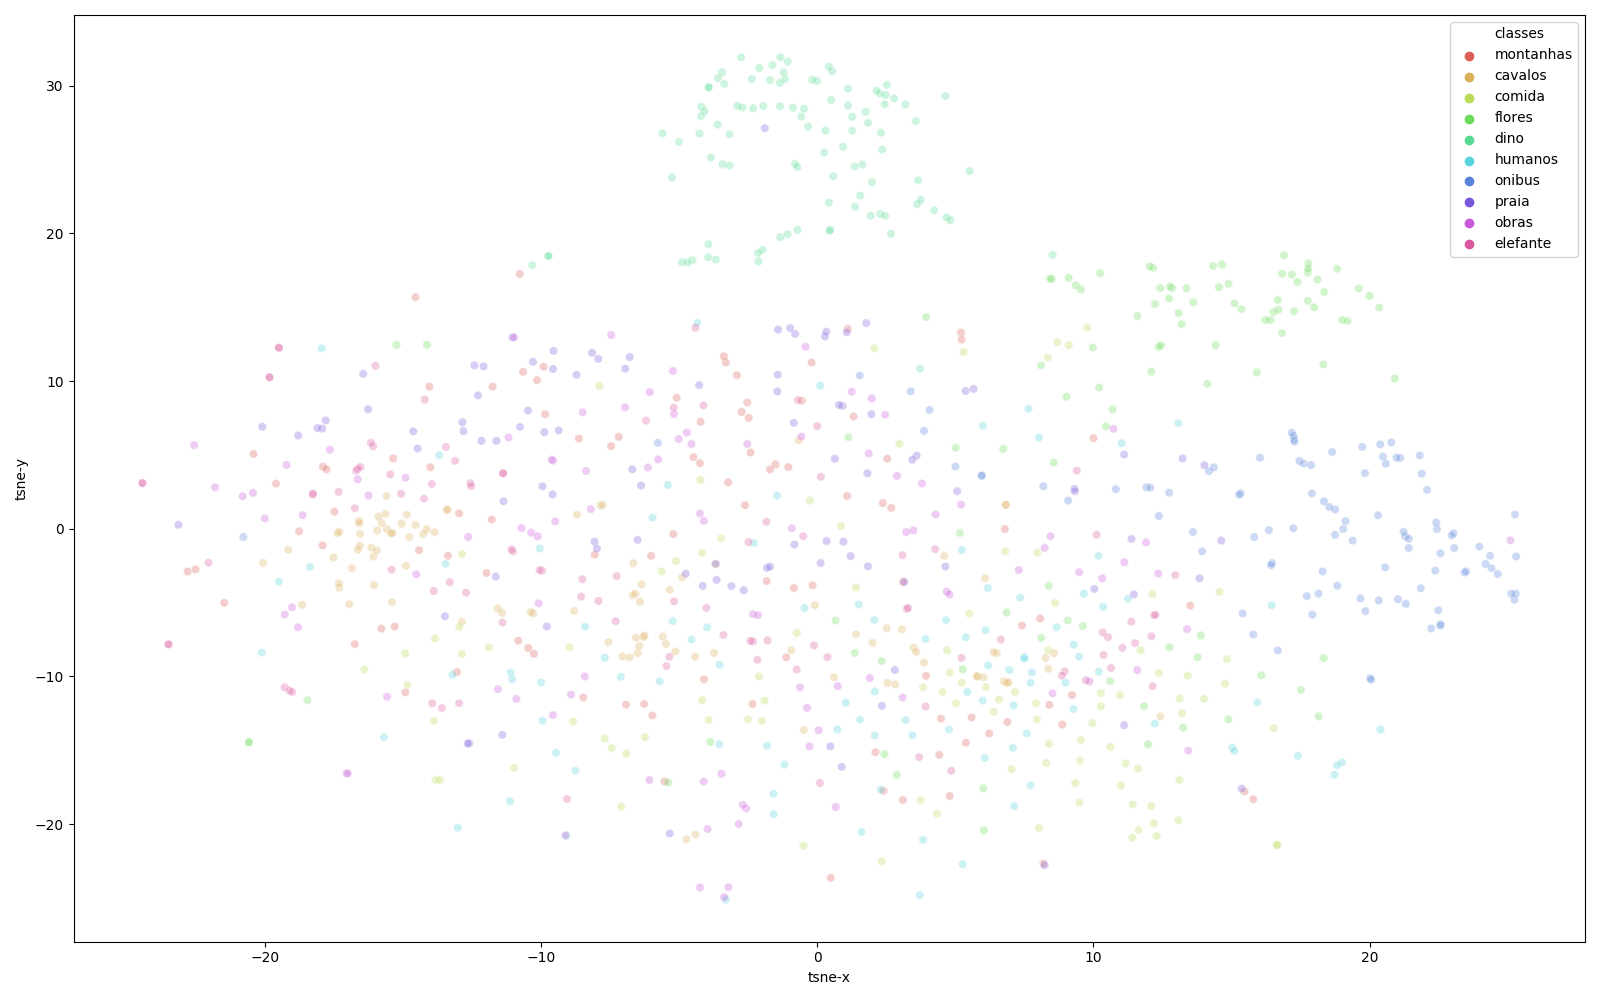
\includegraphics[scale=0.3]{tsne-graph-hand-craft.png}
		\end{center}
		\legend{Fonte: O Autor}
	\end{figure}
	
	\end{anexosenv}
	
	% ----------------------------------------------------------
	% Agradecimentos
	% ----------------------------------------------------------
	
	\section*{Agradecimentos}
	Texto sucinto aprovado pelo periódico em que será publicado. Último 
	elemento pós-textual.
	
\end{document}
